\chapter{体感系统的受体} \label{chap:chap18}
个体感觉方式的神经生理学研究首先在体感系统(希腊语 soma,身体)中进行,该系统传输由分布在全身的受体编码的信息。 
这些身体感觉最早的研究者之一查尔斯·谢林顿 (Charles Sherrington) 指出,体感系统具有三个主要功能:本体感觉、外感觉和内感觉。


本体感觉是自己的感觉(拉丁语proprius,自己的)。 
骨骼肌、关节囊和皮肤中的受体使我们能够有意识地意识到自己身体的姿势和运动,尤其是四肢和头部。 
尽管可以在没有本体感受器的感觉反馈的情况下移动身体的某些部分,但这些运动往往笨拙、协调性差,并且不能充分适应复杂的任务,尤其是在没有视觉引导的情况下。


外部感受是在影响身体时与外部世界直接互动的感觉。 
外部感受的主要模式是触觉,包括接触、压力、抚摸、运动和振动的感觉,用于识别物体。 
一些触觉涉及主动运动组件——抚摸、敲击、抓握或按压——由此身体的一部分相对于另一个表面或生物体移动。 
触觉的感觉和运动成分在大脑中在解剖学上紧密相连,对指导行为很重要。


外部感受还包括热和冷的热感觉。 
热感觉是维持体温接近 37°C (98.6°F) 所需的行为和稳态机制的重要控制因素。 
最后,外部感受包括疼痛感或伤害感受,是对损害或伤害身体的外部事件的反应。 
伤害感受是生存所必需的行动的主要动机,例如战斗或逃跑。


躯体感觉的第三个组成部分,内感受,是身体主要器官系统的功能及其内部状态的感觉。 
内脏受体传递的信息对于调节自主功能至关重要,特别是在心血管、呼吸、消化和肾脏系统中,尽管这些受体记录的大多数刺激不会导致有意识的感觉。 
间感受器主要是通过血气和 pH 值等指标监测器官功能的化学感受器,以及感知组织膨胀(可能被认为是疼痛)的机械感受器。


这组不同的感觉功能似乎不太可能组合形成一个感觉系统。 
我们在介绍性章节中介绍了所有躯体感觉,因为它们是由一类感觉神经元——背根神经节 (DRG) 神经元介导的。 
来自皮肤、肌肉、关节囊和内脏的体感信息由支配四肢和躯干的 DRG 神经元或支配颅骨结构(面部、嘴唇、口腔、结膜和硬脑膜)的三叉感觉神经元传递。 
这些感觉神经元执行两个主要功能:将刺激转导和编码为电信号,以及将这些信号传输到中枢神经系统。


在过去的 10 年里,躯体感觉的研究因三项重要进展而发生了革命性的变化。 
首先,开发具有 DRG 神经元基因表达荧光报告基因的转基因小鼠,使神经科学家能够评估特定受体类别的生理反应及其对身体和中枢神经系统中感觉受体的解剖预测。 
表达基因编码的钙传感器(如 GCaMP6)的单个 DRG 神经元的功能成像可以同时光学记录支配身体特定区域的受体神经元群的活动,从而为分析对体感刺激的整体反应提供有用的工具。 
其次,在体外对分离的 DRG 神经元或在减少的皮肤神经制剂中进行研究,可以对受体反应进行生物物理评估,并对单个体感神经元中表达的离子通道进行表征。 
第三,将压电蛋白离子通道鉴定为哺乳动物机械感受器中触觉和本体感觉的分子传感器,为评估这些通道在触觉、本体感觉和内脏功能中的作用提供了一个新的系统。


在本章中,我们将考虑所有 DRG 神经元的共同原则以及区分它们各自感觉功能的原则。 
我们首先描述周围神经及其组织,然后调查负责每种主要身体感觉的受体类别。 
我们还研究了将各种刺激能量转化为电信号的感觉传导机制。 
然后,我们描述了母体轴突在其感受野中整合来自多个受体的信息,最后讨论了脊髓和脑干中每个亚模态的中央处理中心。 
触觉、疼痛、本体感觉和内脏自主调节的高阶处理将在后面的章节中描述。



\section{背根神经节神经元是体感系统的初级感觉受体细胞}

DRG 神经元的细胞体位于脊神经或脑神经背根的神经节中。 
背根神经节神经元起源于神经嵴,与附近的脊髓节段密切相关。 
DRG 中的单个神经元由于其外围末端的形态学和分子特化而选择性地响应特定类型的刺激。


背根神经节神经元是一种双极细胞,称为伪单极细胞。 
DRG 神经元的轴突有两个分支,一个投射到外围,一个投射到中枢神经系统(图 \ref{fig:18_1})。 
单个 DRG 神经元的外周末端支配皮肤、肌肉、关节囊或内脏,并包含专门用于特定种类刺激的受体。 
受这些感觉末梢支配的身体区域称为皮节(见图 18-13)。 
感觉周围神经末梢在受体形态和刺激选择性方面有所不同,使它们能够检测机械、热或化学事件。 
中央分支终止于脊髓或脑干,形成体感通路中的第一个突触。 
因此,每个 DRG 细胞的轴突作为单一传输线,在受体末端和中枢神经系统之间具有一个极性。 
该轴突称为初级传入纤维。

\begin{figure}[htbp]
	\centering
	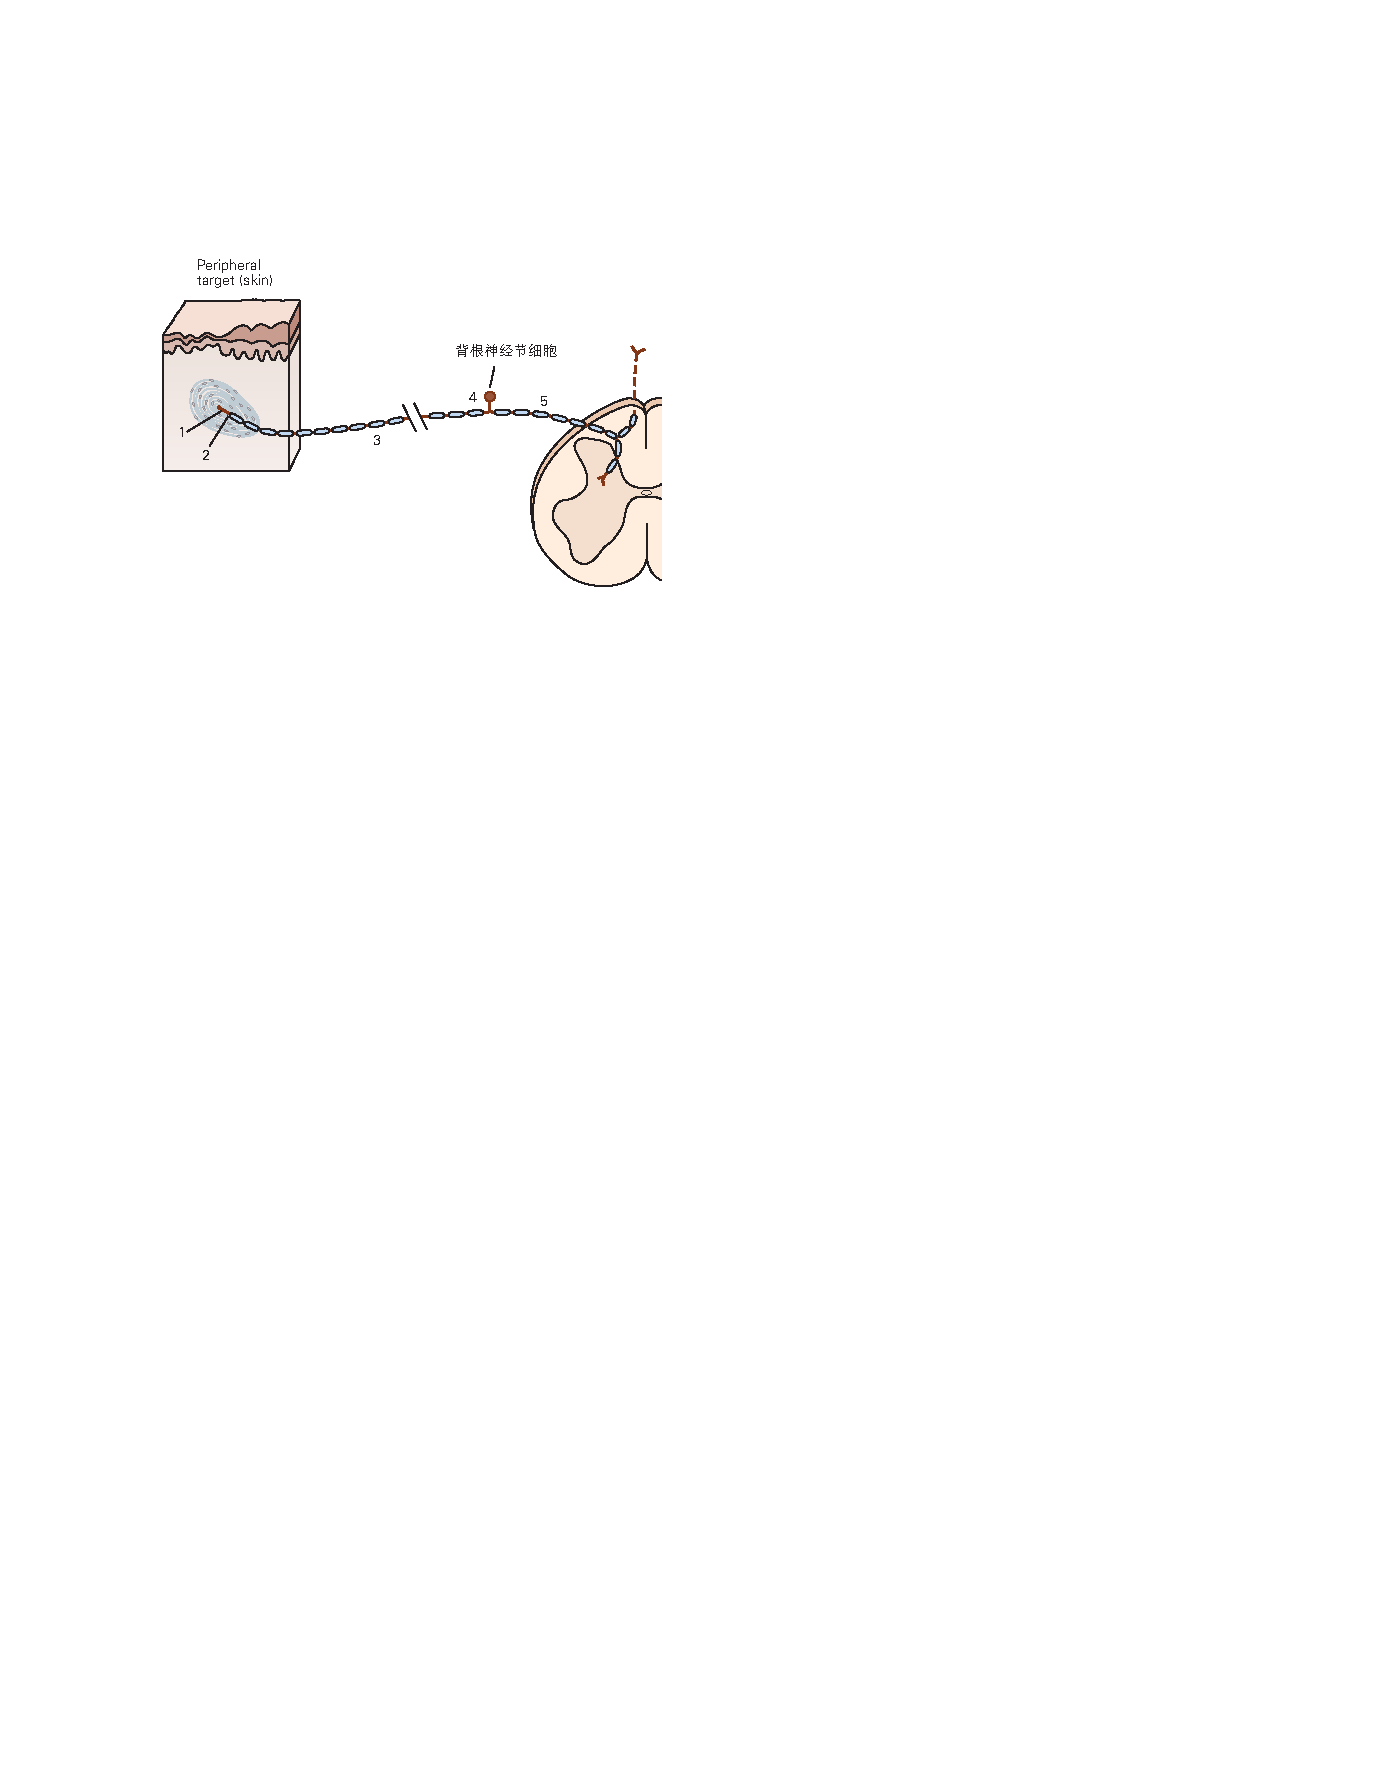
\includegraphics[width=0.5\linewidth]{chap18/fig_18_1}
	\caption{背根神经节神经元是体感系统的初级感觉细胞。 
		细胞体位于与脊髓相邻的背根神经节 (DRG) 中。 
		轴突有两个分支,一个投射到身体,其专用末端包含特定形式刺激能量的受体,另一个投射到脊髓或脑干,传入信号在这里被处理。 
		所有 DRG 神经元都包含五个功能区: 
		1. 皮肤、肌肉或内脏的远端末端包含专门的受体通道,可将特定类型的刺激能量(机械、热或化学)转化为去极化受体电位。 
		DRG 神经元通常具有多个感觉末梢。 
		2. 尖峰生成位点包含电压门控的 Na+ 和 K+ 通道(NaV 和 KV),它们位于受体囊内轴突起始段附近; 它们将受体电位转化为动作电位流。 
		3. 周围神经纤维将动作电位从棘突起始部位传递到背根神经节细胞体。 
		4. DRG 神经元的细胞体包含在与脊髓或脑干相邻的神经节内。 
		5. 脊神经或脑神经将 DRG 或三叉神经元连接到同侧脊髓或脑干。}
	\label{fig:18_1}
\end{figure}


支配身体特定区域(例如拇指或手指)的单个初级传入纤维聚集在一起,形成形成周围神经的轴突束或束。 它们在发育过程中被各种营养因子引导到体内的特定位置,例如脑源性神经营养因子 (BDNF)、神经营养因子 3 (NT3)、神经营养因子 4 (NT4) 或神经生长因子 (NGF)。 
外周神经还包括支配附近肌肉、血管、腺体或内脏的运动轴突。


周围神经或其在大脑中的目标的损伤可能会导致特定肌肉群中不止一种体感亚模式或运动缺陷的感觉缺陷。 
了解体感模式在形态学上的重叠位置和分歧位置,有助于神经系统疾病和功能障碍的诊断。


每个 DRG 神经元可细分为五个功能区:感受区、尖峰生成部位、周围神经纤维、DRG 细胞体和脊髓或脑神经(图 \ref{fig:18_1})。 
位于 DRG 轴突远端的感受区包含专门的受体蛋白,可感知局部环境中的机械力、热事件或化学物质,并将这些信号转化为轴突末端的局部去极化,称为受体电位(参见 图 \ref{fig:3_9} A)。 
这种局部去极化被动地向产生动作电位的中央轴突扩散,通常在初始段(远端到有髓纤维中 Ranvier 的第一个节点)(见图 \ref{fig:3_10} A)。 
足够强度的刺激会产生动作电位,这些动作电位沿着周围神经纤维传递,通过细胞体,并进入终止于脊髓或脑干的中央分支。


DRG 神经元的躯体包含细胞核。 
感觉受体蛋白在体细胞中表达,为体外表征它们的电导特性提供了一个方便的表达系统。 
分离的 DRG 神经元已广泛用于感觉受体电流和电压门控动作电位通道的膜片钳研究。


DRG 神经元在细胞体大小、基因表达谱、轴突传导速度、感觉转导分子、体内神经支配模式和生理功能方面存在差异。 
例如,支配感觉触觉和本体感觉的机械感受器的 DRG 具有最大的细胞体和大的有髓轴突; 它们表达 Npy2r 或小清蛋白 (PV) 等蛋白质(图 \ref{fig:18_2})。 
相比之下,感知温度或刺激性化学物质的 DRG 神经元具有小细胞体和无髓鞘轴突; 它们表达降钙素基因相关肽 (CGRP) 或凝集素 IB4(图 \ref{fig:18_2} C、D)。 
当这些荧光分子标记通过轴突延伸到它们在身体和中枢神经系统中的外周末梢时,David Ginty 及其同事能够表征身体中体感神经末梢的模式(图 \ref{fig:18_2}H)并追踪它们的中枢 投射到脊髓(图 \ref{fig:18_2}G)和脑干。

\begin{figure}[htbp]
	\centering
	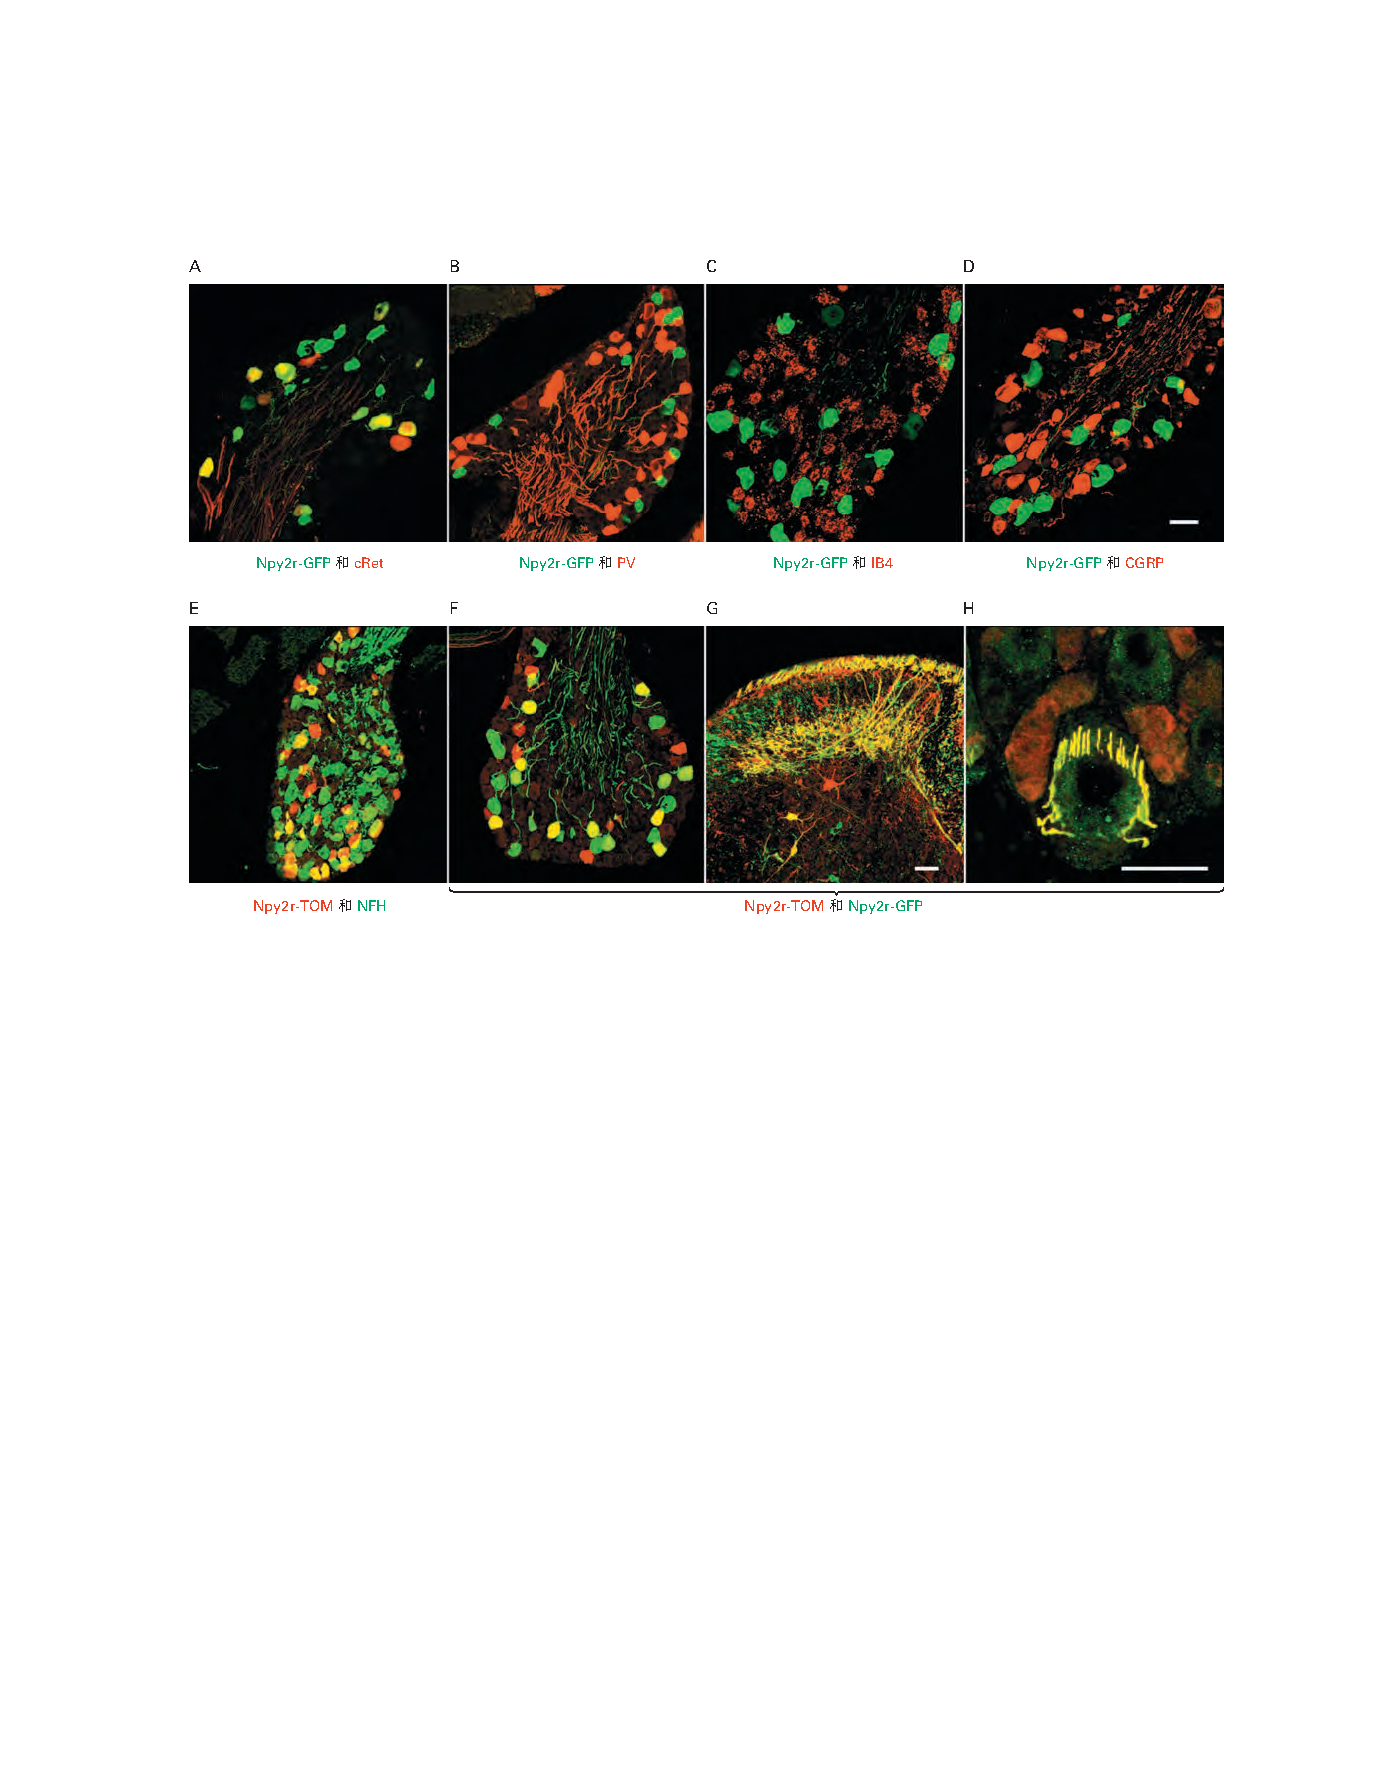
\includegraphics[width=1.0\linewidth]{chap18/fig_18_2}
	\caption{背根神经节神经元的大小、基因表达和皮肤神经支配模式各不相同。 (经许可转载自 Li 等人,2011 年。版权所有 © 2011 Elsevier Inc.)图 A-F 显示通过胸背根神经节对组织切片进行双重免疫染色。 
		这些部分中的单个背根神经节 (DRG) 神经元表达特定类别的体感神经纤维的遗传标记。 
		G 蛋白偶联受体 Npy2r-GFP(绿色)或 Npy2r-TOM(红色)在生理学上标记了 Aβ 快速适应低阈值机械感受器 (Aβ RA-LTMR)。 这些纤维还表达神经丝重链多肽 (NFH),这是重度髓鞘轴突 (E) 的标志物,形成纵向披针形(梳状)末端,围绕着毛茸茸的皮肤中的单个针毛或锥子/紫红色毛发 (H),并终止于层板 III 到 V 的背角 (G)。 
		双标神经元或纤维被染成黄色。 
		A. Aβ RA-LTMR 在发育早期表达受体酪氨酸激酶 Ret(命名为早期 Ret 并染成红色)。 
		大多数这些神经元也表达 Npy2r-GFP(绿色); 表达这两种标记的神经元被染成黄色。 Aβ RA-LTMR 具有中等大小的细胞体。 
		B. Aβ RA-LTMR(绿色)比本体感受器(例如肌梭传入神经和表达小白蛋白的高尔基肌腱器官)具有更小的细胞体(PV,红色)。 
		C、D. Aβ RA-LTMR(Npy2r-GFP,绿色)比释放 ATP 作为共递质(IB4,红色)的无髓鞘嘌呤 C 纤维和表达降钙素基因相关肽(CGRP,红色)的肽能 Aδ LTMR 具有更大的细胞体 . E. 具有大细胞体的重度髓鞘周围神经纤维表达神经丝重链多肽(NFH,绿色)。 
		这些包括 Ia 和 Ib 组肌肉传入神经、Aβ SA-LTMR 和 Aβ RA-LTMR(也标有 Npy2r-tdTom [红色])。 
		只有 Aβ RA-LTMR 表达这两种标记并被染成黄色。 F-H。 
		用 Npy2r-GFP(绿色)和 Npy2r-tdTomato(红色)对胸 DRG 神经元(F)进行双重免疫染色,它们在脊髓背角(G)的第 III 层到 V 层的中枢过程,以及它们在毛囊处的外周披针形末端 在毛茸茸的皮肤切片 (H) 中显示标记的外周和中央 Aβ RA-LTMR 神经元在很大程度上彼此重叠(黄色),并且此类遗传标记可用于追踪感觉神经末梢。}
	\label{fig:18_2}
\end{figure}



\section{周围体感神经纤维以不同的速率传导动作电位}

将尖峰序列从尖峰产生部位传输到中枢神经系统的外周神经通常用作体感受体机制的神经生理学研究的主要记录部位。 
动物的单个周围神经纤维通常从主轴突束中分离出来,并放置在用作记录电极的细线上。 
微电极——由锋利的钨丝或铂丝制成——也已通过皮肤插入人体周围神经(一种称为显微神经造影术的技术),以测量对各种躯体刺激的感觉反应(第 \ref{chap:chap19} 章)。


周围神经纤维根据与轴突直径和髓鞘形成、传导速度以及它们是感觉还是运动相关的特性分为功能组。 
第一个神经分类方案由 Charles Sherrington 于 1894 年设计,他测量了感觉神经中髓磷脂染色的轴突的直径,随后由 David Lloyd 编纂(表 18-1)。 
他们发现了两个或三个重叠的轴突直径组(图 18-3)。 
后来发现这些解剖学分组在功能上很重要。 
肌肉神经中的 I 组轴突支配肌梭受体和高尔基肌腱器官,它们发出肌肉长度和收缩力的信号。 
II 组纤维支配关节囊中的次级纺锤体末梢和受体; 这些受体还介导本体感觉。 
第 III 组纤维、最小的有髓鞘肌肉传入神经和无髓鞘第 IV 组传入神经发出感觉为疼痛的肌肉和关节外伤或损伤信号。


支配皮肤的神经包含两组有髓神经纤维:II 类纤维支配对触觉有反应的皮肤机械感受器,III 类纤维介导热刺激和伤害性刺激,以及多毛皮肤中的轻触。 
无髓鞘的第 IV 组皮肤传入神经与肌肉中的神经传入神经一样,也可介导热刺激和有害刺激。


另一种对周围神经纤维进行分类的方法是基于对整个神经的电刺激。 
在这种广泛使用的诊断技术中,神经传导速度是在放置在周围神经上方皮肤上的成对刺激电极和记录电极之间测量的。 
例如,在研究正中神经或尺神经的传导时,可以将刺激电极放置在手腕上,将记录电极放置在上臂上。 
通过刺激电极施加的短暂电脉冲在神经中引起动作电位。 
短时间后在手臂中记录的神经信号代表了刺激脉冲激发的所有神经纤维的动作电位总和,称为复合动作电位(第 \ref{chap:chap9} 章)。 
随着更多的神经纤维受到刺激,它的振幅会增加; 总的活动大致与活动神经纤维的总数成正比。


强度增加的电刺激首先在最大的轴突中诱发动作电位,因为它们具有最低的电阻,然后逐渐在较小的轴突中诱发动作电位(图 \ref{fig:18_4})。 
大直径纤维传导动作电位的速度更快,因为电流沿轴突流动的内阻较低,而且 Ranvier 节点沿其长度分布较宽(第 9 章)。 大有髓纤维的传导速度(以米/秒为单位)大约是轴突直径(以微米为单位)的六倍,而细有髓纤维的传导速度是轴突直径的五倍。 对于无髓纤维,将轴突直径转换为传导速度的系数为 1.5 至 2.5。

\begin{figure}[htbp]
	\centering
	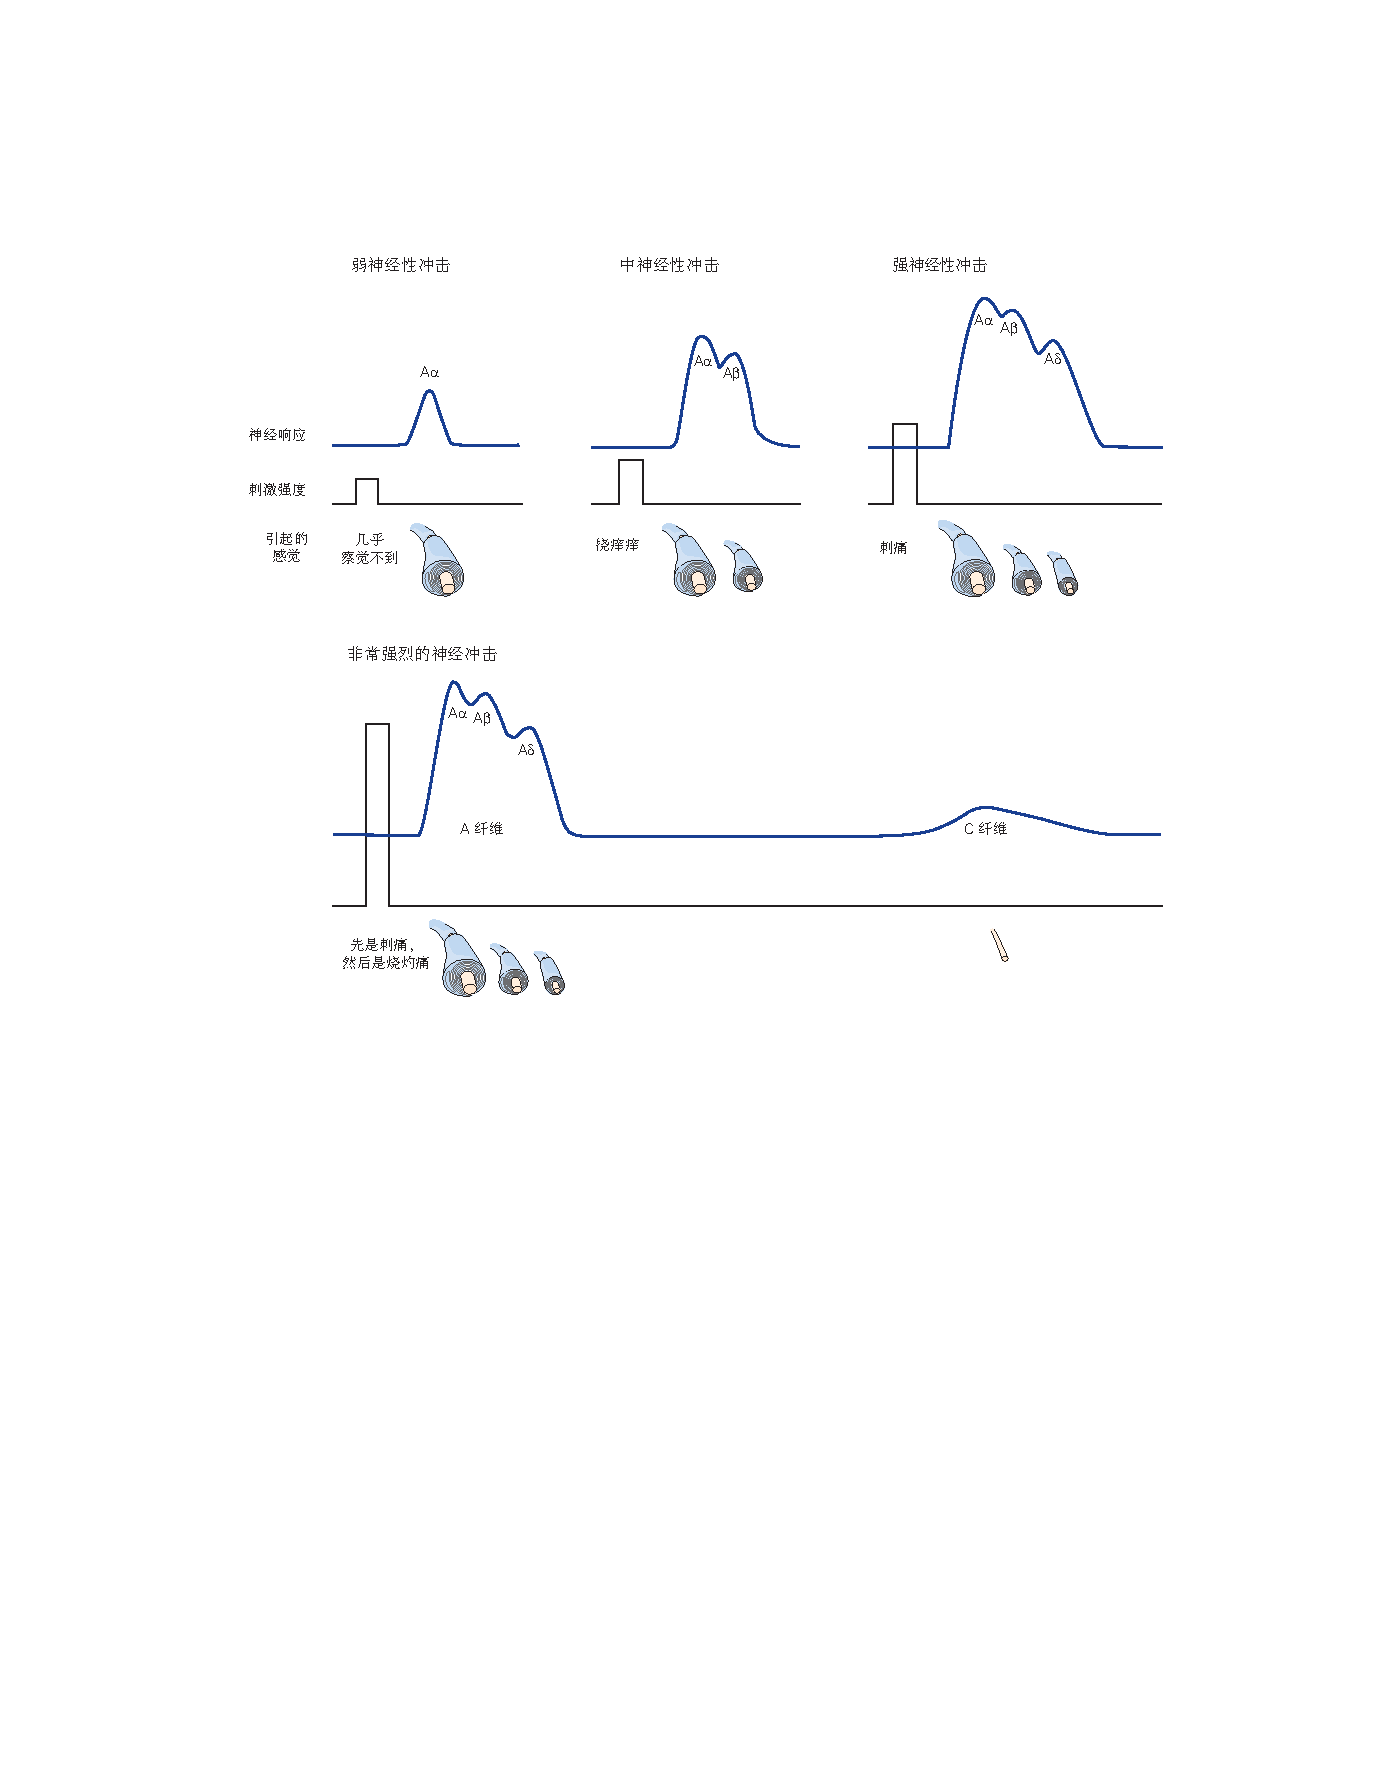
\includegraphics[width=1.0\linewidth]{chap18/fig_18_4}
	\caption{临床上通过复合动作电位测量周围神经的传导速度。 
		不同强度的周围神经电刺激会激活不同类型的神经纤维。 
		由特定电流量刺激的所有神经的动作电位相加以产生复合动作电位。 不同类别的感觉和运动轴突的不同传导速度产生多个峰值。 (改编自 Erlanger 和 Gasser 1938。)}
	\label{fig:18_4}
\end{figure}


在刺激伪影之后,复合动作电位中记录的最早神经信号出现在传导速度大于 90 m/s 的纤维中。 称为 Aα 波(图 \ref{fig:18_4}),该信号反映了 I 组纤维和支配骨骼肌的运动神经元中产生的动作电位。 在受神经支配的区域中,受试者几乎无法感知到这种感觉。

随着更多大纤维被募集,出现第二个信号,即 Aβ 波。 该成分对应于皮肤或肌肉神经中的 II 组纤维,这些神经支配调节触觉和本体感觉的机械感受器,并且随着电击强度的增加而变大。 在较高的电压下,当较小的 Aδ 范围内的轴突被募集时,刺激会变得疼痛,类似于静电产生的电击。 足以激活无髓鞘 C 纤维的电压会引起灼痛感。 正如我们将在本章后面了解到的那样,一些 Aδ 和 C 纤维也会对毛茸茸的皮肤上的轻触做出反应,但是当整个神经受到电刺激时,这种温和的触觉刺激会被同时激活的痛觉纤维所掩盖。 刺激支配肌梭梭内纤维的运动神经元(参见图 18-9)会引发称为 Aγ 波的中间小波,但这通常很难辨别,因为这些运动神经元的传导速度与 Aβ 和 Aδ 感觉轴突的传导速度重叠 . 这些周围神经纤维直径和传导速度的差异使得触觉和本体感觉信号比有害或热信号更早到达脊髓和更高的大脑中枢。

临床医生利用各种传入纤维传导速度的已知分布来诊断导致感觉纤维退化或运动神经元丢失的疾病。 在某些情况下,周围神经轴突的丢失是选择性的; 例如,在糖尿病的神经病变特征中,大直径感觉纤维退化。 这种选择性丧失反映在复合动作电位适当峰值的减少、神经传导的减慢以及相应的感觉能力的减弱上。 同样,在多发性硬化症中,中枢神经系统中大直径传入纤维的髓鞘退化会导致神经传导减慢,如果足够严重,还会导致神经传导失败。


\section{体感系统使用多种特殊受体}
单个 DRG 神经元的功能特化是由发生在身体远端神经末梢的感觉转导的分子机制决定的。 当躯体受体被适当的刺激激活时,其感觉末端通常会去极化。 去极化的幅度和时间进程反映了刺激的强度及其持续时间(参见图 3-9A)。 足够强度的刺激会产生动作电位,这些动作电位会沿着 DRG 神经元轴突的外周分支传递到终止于脊髓或脑干的中央分支。

介导触觉和本体感觉的感觉神经元终止于非神经囊(图 \ref{fig:18_1})或在毛囊(图 18-2H)或梭内肌纤维(见图 18-9A)周围形成形态独特的末端。 他们感觉到缩进或拉伸他们的接受表面的机械刺激。 相比之下,检测有害、热或化学事件的神经元的外周轴突具有未覆盖的末端,具有多个终止于表皮或内脏的分支。

几种不同的形态学特化受体是各种体感亚模式的基础。 例如,支配手部皮肤的正中神经和一些控制手部的肌肉包含数以万计的神经纤维,可分为 30 种功能类型。 其中,22 种类型是传入纤维(感觉轴突将冲动传导至脊髓),8 种类型是传出纤维(运动轴突将冲动从脊髓传导至骨骼肌、血管和汗腺)。 传入纤维传递来自对不同类型的皮肤变形敏感的八种皮肤机械感受器的信号; 五种本体感受器发出有关肌肉力量、肌肉长度和关节角度的信息; 报告接触皮肤的物体温度的四种温度感受器; 以及四种发出潜在伤害性刺激信号的伤害感受器。 表 18-2 中列出了每个子模态中的主要受体组。

\subsection{机械感受器介导触觉和本体感受}
机械感受器感知周围组织的物理变形。 机械扩张——例如皮肤压力、肌肉拉伸、直接作用于细胞膜的吸力或组织的渗透性肿胀——通过刺激膜中机械感受器离子通道的物理作用转化为电能。 机械刺激使受体蛋白变形,从而打开拉伸敏感离子通道并增加使受体神经元去极化的非特异性阳离子电导(参见图 3-9A)。 去除刺激可以减轻受体上的机械应力,并允许拉伸敏感通道关闭。

已经提出了用于激活机械感受器离子通道的各种机制。 一些机械感受器似乎对通过质膜脂质的张力或变形传递的力作出反应,这种机制称为来自脂质的力(图 18-5A)。 在这里,膜脂的变形改变了细胞表面的曲率,将受体蛋白中的疏水残基暴露给膜磷脂,从而打开通道孔以供阳离子流动。 这可能是检测细胞肿胀的机制,细胞肿胀在渗透压调节或由于流体流动改变引起的血管壁剪切应力变化中起着重要作用。

另一种假设的机械感受器激活机制涉及通过结构蛋白将通道蛋白连接到周围组织,一种称为细丝力的机制(图 18-5B)。 在这种排列中,通过组织的直接压力或横向拉伸施加到皮肤或肌肉的机械力会扭曲细胞外基质或细胞内细胞骨架蛋白(肌动蛋白、整合素、微管)。 这些束缚分子与受体通道蛋白相互作用,改变它们的构象,并打开阳离子通道。 与通道蛋白的细胞外连接是有弹性的,通常表示为弹簧门。 该模型中的直接通道门控可能是由拉伸细胞外连接蛋白的力产生的。 当力被移除时,通道关闭。 这种类型的直接通道门控被内耳的毛细胞和皮肤中的一些触觉感受器使用。

值得注意的是,虽然 Edgar Adrian 和 Yngve Zotterman 在 1920 年代首先研究了皮肤触觉的受体末端器官,并且在 1960 年代从肠系膜(Pacinian 小体)分离的触觉感受器记录了受体电位,但几乎没有达成共识 关于哺乳动物触摸中机械感觉的分子生物学。 领先的候选者来自无脊椎动物模型生物,例如线虫秀丽隐杆线虫,其触觉感受器被确定为离子通道变性蛋白超家族的成员,类似于脊椎动物上皮 Na+ 通道(DEG/ENac 通道)。 其他候选分子包括 TRPV4 受体(也参与热感觉的瞬时受体电位 [TRP] 受体的成员)和 NOMPC,TRPN 家族的果蝇成员。 然而,这些分子不在哺乳动物 DRG 神经元中表达。

跨膜离子通道的压电蛋白家族最近被 Ardem Patapoutian 及其同事鉴定为哺乳动物机械感受的分子介质。 Piezo1 蛋白由大约 2,500 个氨基酸组成,至少有 26 个跨膜 α 螺旋(图 18-6A)。 离子通道是由三个相同的 Piezo 蛋白亚基形成的三聚体,每个 Piezo 蛋白的 C 末端有两个成孔 α 螺旋。 亚基的 N 端形成螺旋桨状结构(图 18-6B),这被认为与耦合机械刺激与通道门控有关。 压电蛋白形成非特异性阳离子可渗透通道,可传导兴奋性去极化电流。

Piezo 蛋白的两种不同亚型用作机械传感器:Piezo1 主要存在于非神经组织中,例如血管、肾脏和膀胱中的上皮细胞,以及红细胞。 Piezo2 在调节触觉和本体感觉的机械感觉 DRG 和三叉神经神经元中表达,在支配肺部平滑肌的迷走神经传入神经中表达,它们通过感知肺部伸展来调节 Hering-Breuer 反射(第 32 章)。

\subsection{专门的终末器官有助于机械感觉}
除了在远端神经末梢表达的离子通道的分子组成外,周围组织的成分如上皮细胞或肌纤维在机械传导中也起着重要作用。 围绕 DRG 神经元神经末梢的特殊非神经终末器官必须以特定方式变形以激发纤维。 例如,个体机械感受器选择性地响应压力或运动,从而检测施加到皮肤、关节或肌肉纤维的力的方向。 末端器官还可以放大或调节受体轴突对机械位移的敏感性。

皮肤中的特殊上皮细胞——例如默克尔细胞、毛囊内衬的上皮细胞和形成无毛皮肤指纹的乳头状脊——在触觉中起着重要的辅助作用。 这些末端器官中研究得最好的是默克尔细胞——感觉上皮细胞,在表皮-真皮交界处与大直径 (Aβ) 感觉神经轴突的末端形成紧密接触,形成默克尔细胞-神经突复合物。 Merkel 细胞聚集在多毛皮肤表皮的肿胀处,称为触摸圆顶(图 18-7A),在无毛皮肤中靠近指纹脊的中心(见图 19-3)。 当探头接触触摸圆顶时,感觉神经会响应一系列动作电位,其频率与施加到皮肤上的压力的速度和幅度成正比(图 18-7A2)。 这些尖峰序列通常在整个刺激期间持续,并被称为缓慢适应,因为放电持续长达 30 分钟。 同样,感觉神经称为 SA1 纤维(缓慢适应 1 型纤维)。

默克尔细胞在触觉方面的感受功能类似于耳蜗中的听觉毛细胞(第 26 章)和舌头中的味觉细胞(第 32 章)。 体外研究的 Merkel 细胞对压力或吸力等机械力作出反应,去极化电流在时间过程和电导方面与孤立的 DRG 神经元中诱发的电流相似。 它们表达突触释放蛋白并包含在持续压力下释放兴奋性神经递质的囊泡。 Merkel 细胞表达 Piezo2 蛋白,并在压力刺激下显示细胞质 Ca2+ 水平升高。

Merkel 细胞对触觉生理反应的重要性在未能在表皮中形成 Merkel 细胞的小鼠(Atoh1 条件性基因敲除小鼠)中可见。 与野生型相比,这些动物中 SA1 纤维的放电率在振幅和持续时间上有所降低。 这些实验表明默克尔细胞负责对静态触摸的持续反应。 最近,Ellen Lumpkin 及其同事使用 Merkel 细胞的光遗传学刺激而不是直接对皮肤施加压力来证明支配触摸圆顶的 SA1 纤维使用双重机制来感知皮肤上的压力(图 18-7B)。 对触摸的初始动态响应主要是由流过 SA1 神经末梢 Piezo2 通道的电流产生的。 随后的静态反应是由 Merkel 细胞的兴奋性突触传递引起的,Merkel 细胞表达 Piezo2 通道并在持续对皮肤施加压力时不断释放神经递质。

从皮肤表面突出的毛发提供了另一组重要的触摸端器官。 感觉毛发纤维对运动极其敏感。 微风或吹气使头发偏转会从毛囊传入纤维中激发一种或多种动作电位。 人类可以感知单根毛发的运动,并将这种感觉定位于毛发根部,也就是毛发从皮肤中露出来的地方。 感觉毛发具有重要的保护功能,因为它们会在物体、其他生物体或环境中的障碍物影响身体之前检测到它们。 毛发或感觉触角检测重要的物体特征,如纹理、曲率和刚度,这些特征有助于识别朋友或敌人。 这些神经元被命名为快速适应低阈值机械感受器 (RALTMR),因为当头发受到外力移动时,它们会对轻柔的触摸或头发运动做出短暂的尖峰脉冲响应。

头发嵌入称为毛囊的皮肤内陷中。 在哺乳动物皮肤中发现了三种类型的毛发(图 18-8A)。 最大、最长和最硬的毛发(称为针毛)在发育过程中最先从皮肤长出。 针毛由直径最大、传导速度最快的感觉神经纤维(Aβ 型)支配; 这些纤维在毛发周围的毛囊表皮形成披针形(梳状)末端(图 18-2H)。 Aβ RA-LTMR 神经纤维还支配具有披针形末梢的中等大小的毛发(称为锥形毛/桃红毛)。 Awl/auchene 毛发具有三重神经支配:它们为快速传导 (Aβ) 有髓纤维提供输入; 直径更小、传导速度更慢的有髓 (Aδ) 纤维; 和无髓鞘的 C 纤维。 最小和最多的毛发(称为之字形或绒毛)也受 Aδ 和 C 纤维支配。

直到最近,Aδ 和 C 纤维还被认为只调节热觉或痛觉。 然而,Johan Wessberg、Håkan Olausson 和 Åke Vallbo 对人类进行的显微神经造影研究表明,毛茸茸的皮肤也受到无髓鞘 C-LTMR 纤维的支配,这些纤维对缓慢移动的触觉刺激做出反应,并被认为可以调节社交或愉悦的触觉。 它们还可能在脊髓背角的疼痛抑制中发挥作用。

皮肤中毛囊的神经支配模式说明了身体感觉神经支配的两个重要原则:收敛和发散。 皮肤中的每个毛囊都为多种感觉传入纤维提供输入。 这种重叠模式提供了一小块皮肤的感觉输入冗余。 共享的通信线路支配每个毛囊,而不是单一的标记线路。 因此,来自皮肤的触觉信息由一组感觉神经元并行传输。

由 DRG 神经元的感觉神经末梢支配的皮肤区域定义了细胞的感受野,即可以激发细胞的身体区域。 每条感觉神经纤维都从广泛的皮肤区域收集信息,因为它的远端末端有多个可以独立激活的分支。 这种形态使每条传入纤维能够为大脑提供独特的感觉输入模式。

图 18-8B 说明了不同类别的 DRG 神经元所包含的感受野大小和区域的多样性。 由于触觉感受野的面积很大,轻柔的触摸会在接触部位激发许多不同的感觉纤维,每一种都传达一种特定的感觉信息。 最小的触觉感受野是由 SA1 纤维支配的触摸圆顶(参见图 19-8B Aβ SA1)。 单个 SA1 纤维支配触摸圆顶中的所有 Merkel 细胞,通常从相邻皮肤区域的一到三个触摸圆顶收集信息。 由单个 RA 纤维支配的毛囊分布得更远,感觉末梢的大小略有不同,直径最大的 Aβ 纤维包含最小的毛囊感受野(参见图 19-8B Aβ RA)。 皮肤中最大的感受野是 Aβ 场受体(参见图 19–8B Aβ 场)。 这些纤维在毛囊周围形成圆周末端,但对毛发运动或吹气没有反应。 取而代之的是,场感受器会在其感受区内对抚摸或拉伸皮肤做出反应。 场感受器也会因拉扯头发或强力压力等疼痛刺激而兴奋,这表明它们也可能介导机械疼痛的感觉。

\subsection{本体感受器测量肌肉活动和关节位置}
肌肉和关节中的机械感受器传达有关身体姿势和运动的信息,从而在本体感觉和运动控制中发挥重要作用。 感觉神经末梢与骨骼肌、肌腱、关节囊和皮肤的机械耦合被认为是本体感觉的基础。 这些受体包括两种类型的肌肉长度传感器,即 Ia 型和 II 型肌梭末梢; 一个肌肉力传感器,高尔基肌腱器官; 关节囊受体,可传导关节囊中的张力; 和感觉皮肤在关节上伸展的 Ruffini 结尾。

肌梭由一束细肌纤维或梭内纤维组成,它们与较大的肌肉纤维平行排列并封闭在胶囊内(图 18-9A)。 由于神经末梢中的机械感受性离子通道,梭内纤维被一对感觉轴突缠绕在一起,这些轴突检测肌肉拉伸。 梭内肌还接收来自调节收缩力和受体敏感性的运动轴突的输入。 (有关肌梭的详细信息,请参见方框 32-1。)

尽管肌梭传入纤维的受体电位和放电率与肌肉长度成正比(图 18-9B),但这些反应可以通过大脑中调节梭内肌肉收缩的更高中枢来调节。 因此,纺锤体传入纤维能够对内部产生的随意运动的幅度和速度以及外力造成的被动肢体位移进行编码(第 32 章)。

位于骨骼肌和肌腱交界处的高尔基肌腱器官测量肌肉收缩产生的力。 (有关高尔基肌腱器官的详细信息,请参见方框 32-4。)尽管这些受体在调节肌肉力量的反射回路中起着重要作用,但它们似乎对肌肉活动的有意识感觉贡献不大。 肌肉疲劳或部分瘫痪的心理物理学实验表明,感知的肌肉力量主要与集中产生的力量有关,而不是与实际肌肉力量有关。

Ardem Patapoutian 及其同事最近的研究表明,Piezo2 介导来自肌梭和高尔基肌腱器官的传入纤维传输的信号,因为这些纤维在其远端和细胞体中表达 Piezo2 蛋白。

关节受体在关节角度的姿势感觉中几乎没有作用。 相反,对近端关节(例如肘部或膝盖)角度的感知取决于来自肌梭感受器的传入信号和传出运动命令。 此外,手指位置和手形的有意识感觉取决于皮肤牵张感受器和肌梭。

\subsection{热感受器检测皮肤温度的变化}
虽然手持物体的大小、形状和质地可以通过视觉和触觉来理解,但物体的热特性是独一无二的体感。 人类识别四种不同类型的热感觉:冷、凉、暖和热。 这些感觉是由大约 32°C (90°F) 的正常皮肤温度与空气或接触身体的物体的外部温度之间的差异引起的。 与疼痛和瘙痒的其他原发病方式一样,温度感由多种受体类型的组合代码介导,由小直径传入纤维传递。

虽然人类对皮肤温度的突然变化非常敏感,但我们通常不会意识到皮肤血管扩张或收缩以排出或保存体温时皮肤温度的大幅波动。 如果体表温度变化缓慢,我们不会意识到 31° 至 36°C(88–97°F)范围内的变化。 在 31°C (88°F) 以下,感觉从凉爽发展为寒冷,最后在 10° 至 15°C (50–59°F) 时开始发展为疼痛。 高于 36°C (97°F) 时,感觉会从温暖变为热,然后从 45°C (113°F) 开始变为疼痛。

热感觉由表皮中的游离神经末梢介导。 这些神经纤维发出信号的温度范围由小直径 DRG 神经元的远端神经末梢和细胞体中表达的受体分子的分子组成决定。 David Julius 及其同事的研究表明,热刺激会激活这些神经元中特定类别的瞬时受体电位 (TRP) 通道(图 18-10)。 TRP 通道由与产生动作电位的电压门控通道属于同一基因超家族的基因编码(第 8 章)。 它们形成介导内向去极化电流的非选择性阳离子通道。 TRP 通道包含四个相同的蛋白质亚基,每个亚基包含六个跨膜 α-螺旋,在第五和第六螺旋之间有一个成孔元件。 单个 TRP 受体的区别在于它们对热或冷的敏感性,当超过其热阈值时,显示出对阳离子的电导率急剧增加。 它们的名称指定了 TRP 受体的遗传亚家族和成员编号。 示例包括 TRPV1(对于 TRP vanilloid-1)、TRPM8(对于 TRP melastatin-8)和 TRPA1(对于 TRP ankyrin-1)。

两类 TRP 受体在寒冷温度下激活,在变暖下失活。 TRPM8 受体对低于 25°C (77°F) 的温度有反应; 这样的温度被认为是凉爽或寒冷的。 TRPA1 受体的热阈值低于 17°C (63°F); 这个范围被描述为寒冷或寒冷。 TRPM8和TRPA1受体均在高阈值冷受体末端表达,但只有TRPM8受体在低阈值冷受体末端表达。

来自低阈值冷感受器的热信号通过表皮内具有无髓末端的小直径有髓鞘 Aδ 纤维传输。 这些纤维表达瞬时受体电位通道 TRPM8 并对应用于皮肤的薄荷醇作出反应。 冷感受器对皮肤温度突然下降的敏感度大约是对逐渐变化的敏感度的 100 倍。 这种对变化的极端敏感性使人类能够从远处打开的窗户检测到气流。

四种类型的 TRP 受体被温暖或高温激活,并被冷却灭活。 TRPV3 受体在暖型纤维中表达; 它们对高于 35°C (95°F) 的皮肤升温做出反应,并产生从暖到热的各种感觉。 TRPV1 和 TRPV2 受体对超过 45°C (113°F) 的温度有反应并介导灼痛感; 它们在热伤害感受器中表达。 TRPV4 受体在 27°C 以上的温度下活跃,并发出正常皮肤温度的信号。

暖感受器位于终止于真皮的 C 纤维末端。 与冷感受器不同,暖感受器更像是简单的温度计。 它们的放电率随着皮肤温度的升高而单调上升,直至达到疼痛阈值,然后在更高的温度下达到饱和。 与冷感受器相比,暖感受器对皮肤温度的快速变化不太敏感。 因此,人类对变暖的反应不如对冷却的反应; 即使是最敏感的受试者,检测皮肤突然变暖的阈值变化也约为 0.1°C。

热伤害感受器在超过 45°C (113°F) 的温度下被激活,并在皮肤冷却时失活。 高温引起的灼痛是由有髓 Aδ 纤维和无髓 C 纤维共同传递的。

TRP 受体在热感觉中的作用最初是通过分析辣椒素和薄荷醇等天然物质发现的,这些物质在应用于皮肤或皮下注射时会产生灼烧感或凉爽感。 辣椒素是辣椒中的活性成分,已被广泛用于激活伤害性 C 纤维传入神经,介导灼痛感。 这些研究表明,各种 TRP 受体还结合其他分子,这些分子会引起疼痛感,例如毒素、毒液以及患病或受伤组织释放的物质。 TRPA1 受体结合辛辣物质,例如辣根(芥末)、大蒜、洋葱和类似的葱属植物。 这些物质表现为刺激物,可能通过共价修饰 TRPA1 蛋白中的半胱氨酸而产生疼痛或瘙痒。

TRP 通道是多模式感觉整合器,因为蛋白质的不同部分直接响应温度、pH 值或渗透压的变化; 存在有毒物质,例如辣椒素或毒素; 或被细胞内第二信使磷酸化(见图 20-2)。 第 20 章详细介绍了它们的分子结构和在疼痛中的作用。

\subsection{伤害感受器介导疼痛}
对可能损伤组织的刺激有选择性反应的受体称为伤害感受器(拉丁语 nocere,伤害)。 它们直接对机械和热刺激作出反应,并通过从受创伤组织中的细胞释放的化学物质间接对其他刺激作出反应。 伤害感受器发出即将发生的组织损伤信号,更重要的是,它们不断提醒组织已经受伤,必须加以保护。

疾病或创伤导致的主要器官系统功能异常会引起有意识的疼痛感。 我们对疼痛神经机制的大部分了解都来自对皮肤伤害感受器的研究,因为在皮肤神经中研究这些机制比在内脏神经中更容易研究。 然而,内脏痛的神经机制与身体表面疼痛的神经机制相似。

皮肤、肌肉、关节和内脏感受器中的伤害感受器根据其传入纤维的髓鞘形成分为两大类。 由薄髓鞘 Aδ 纤维支配的伤害感受器产生短潜伏期疼痛,被描述为尖锐和刺痛。 大多数被称为机械伤害感受器或高阈值机械感受器 (HTMR),因为它们会被刺入、挤压或捏住皮肤的尖锐物体(图 18-11)或通过拉动多毛皮肤中的毛发而兴奋。 许多这些纤维还会对 45°C(113°F)以上的温度产生反应,从而灼伤皮肤; 这些 Aδ 纤维还表达热敏 TRPV2 通道。

受 C 纤维支配的伤害感受器会产生弥漫性局限性且难以耐受的钝痛、灼痛。 最常见的类型包括多模式伤害感受器,它们对各种有害的机械、热和化学刺激做出反应,例如捏或刺、有害的热和冷,以及应用于皮肤的刺激性化学物质。 如第 20 章所述,大多数 C 多峰伤害感受器表达 TRPV1 和/或 TRPA1 受体。 人体对这些纤维的电刺激会引起长时间的灼痛感。 在内脏中,伤害感受器被膨胀或肿胀激活,产生剧烈疼痛的感觉。

\subsection{痒是一种独特的皮肤感觉}
痒是一种常见的感觉体验,局限于皮肤、眼结膜和粘膜。 它与疼痛有一些共同的特性,直到最近,它还被认为是由伤害感受纤维的低放电率引起的。 就像疼痛一样,无论其强度如何,瘙痒本质上都是令人不快的。 即使以引起疼痛为代价,我们也试图通过抓挠来消除它。

Diana Bautista 和 Sarah Wilson 最近的研究表明,表达 TRPV1 和 TRPA1 受体的 C 纤维介导由瘙痒(产生瘙痒)剂诱发的瘙痒感。 由皮内注射组胺或通过释放内源性组胺的程序引起的瘙痒会激活一部分表达 TRPV1 的神经元,这些神经元也含有 H1 组胺受体; 这些瘙痒感会被抗组胺药阻断。 组胺非依赖性瘙痒似乎是由表达 TRPA1 通道的 C 纤维 DRG 介导的。 该通路中的瘙痒感是由皮肤干燥或与 Mas 相关 G 蛋白偶联受体 (Mrgpr) 家族成员结合的瘙痒原触发的,例如抗疟药氯喹。

当 TRPA1 受体还参与感知有害的寒冷温度(<15°C)时,它们如何调节瘙痒? 为什么一些表达 TRPV1 的纤维介导瘙痒感而不是热毒感? 答案在于小直径感觉神经纤维对组合代码的使用。 例如,当 TRPA1 和 TRPM8 受体都处于兴奋状态时,会感觉到有害的寒冷,而当 TRPM8 受体处于沉默状态时,会感觉到瘙痒。 同样,当表达 TRPV1、TRPV2 和 TRPV3 的纤维被共同激活时,会感觉到热痛,但当只有表达 TRPV1 的纤维有反应而 TRPV2 和 TRPV3 受体处于沉默状态时,可能会感觉到痒。 使用多个受体的类似组合代码通常被其他化学感官(例如嗅觉和味觉)使用。

\subsection{内脏感觉代表五脏六腑的状态}

本能感觉很重要,因为它们驱动对生存至关重要的行为,例如呼吸、进食、饮水和繁殖。 前面描述的用于研究背根和三叉神经节中的触觉、疼痛、热感觉和本体感觉的相同分子遗传策略已被用于对迷走神经感觉神经节中的内脏传入进行分类。 Stephen Liberles 及其同事最近分析了迷走神经感觉神经节(结节/颈静脉复合体)中的感觉反应,该神经节接收来自肺、心血管、免疫或消化系统的机械感觉或化学感觉信息。

迷走神经传入纤维表达多种 G 蛋白偶联受体 (GPCR),这些受体已用荧光抗体标记,以识别其在特定内脏中的外周感觉受体位点,并标记其独特的中央投射到孤立细胞核中的特定区域 髓质束中。 通过在已识别的迷走神经节神经元中表达钙瞬变 (GCaMP) 的遗传标记,Liberles 及其同事测量了它们对机械刺激的生理反应,例如拉伸或它们被营养素或胃激素(5-羟色胺、胰高血糖素样肽 1 或胆囊收缩素)激活。 标记特定迷走神经传入的能力为分析内脏功能的神经调节和追踪用于调节这些重要身体功能的通路提供了重要工具。

尽管它们的细胞体似乎随机散布在迷走神经核中,但单个迷走神经元在特定器官系统中执行不同的感觉功能。 例如,对已识别的迷走神经感觉神经元进行光遗传学刺激表明,至少有两个控制呼吸的迷走神经元群。 表达 GPCR P2ry1 的神经元会诱发呼吸暂停,在呼气时将肺困住,而表达 GPCR Npy2r 的神经元会产生快速浅呼吸。 刺激这些神经元对心率或消化功能没有影响。 另一组 GPCR 用于标记调节胃肠功能的神经元。 一组胃传入是感知胃和上肠扩张并调节胃动力的机械感受器,而其他胃传入是感知肠道中特定营养素并帮助其吸收的化学感受器。

\section{动作电位代码将体感信息传递给大脑}
在前面的部分中,我们了解到各种刺激,如机械力、温度和各种化学物质,与 DRG 神经元远端轴突末端的受体分子相互作用,产生感觉末梢的局部去极化。 如第 17 章所述,这些受体电位被转换为动作电位的数字脉冲代码,以传输到中枢神经系统。

周围神经纤维的感觉末端区域通常没有髓鞘,并且不表达构成动作电位生成基础的电压门控 Na+ 和 K+ 通道。 例如,毛囊传入的披针形末端是无髓鞘的(图 18-2H)。 这种设计通过将高度分支的末端膜区域专用于感觉转导通道(例如 Piezo2 或 TRP 受体)来优化感受野中的信息收集。

有髓纤维中最远端的动作电位离子通道通常位于初始髓鞘段附近(见图 3-10)或无髓纤维中分支的交叉点。 这对信息传输具有重要影响。 如果参与动作电位生成的通道不存在于接受终端,则来自多个分支的去极化感觉信号可以更容易地累加,因为动作电位的再生特性和电压门控 Na+ 通道随后的失活。 来自后激活受体的感觉信息可能会因与沿纤维另一分支传播的向后传播动作电位的碰撞而消失。 因此,沿着初级传入轴突传输的信号可能是感官刺激的非线性反射,反映了来自多个分支的激发的空间总和或对后期产生的活动的赢者通吃抑制。 不同神经突分支的顺序激活还可以通过生成长串动作电位来帮助检测移动刺激,前提是个体末梢以最佳速率受到刺激,这样它们的反应就不会被其他分支中较早产生的尖峰分流。

沿周围神经的动作电位传递取决于轴突是有髓鞘还是无髓鞘以及每根神经纤维中电压依赖性 NaV 和 KV 通道的特定亚类的表达。 Steven Waxman 及其同事报告说,支配本体感受器和低阈值机械感受器 (LTMR) 的大直径 Aα 和 Aβ 纤维主要表达 NaV1.1 和 NaV1.6 亚型; 这些纤维通常以高速率激发动作电位,部分原因是它们还表达能够使轴突快速复极化的 KV1.1 和 KV1.2 通道。 介导痛痒感觉的小直径外周神经表达 NaV1.7、NaV1.8 和 NaV1.9 通道。 后两种 NaV 亚型具有促进重复放电的动力学和电压敏感性,从而增强疼痛感:NaV 1.8 通道在动作电位期间不完全失活并在它们之后迅速恢复; NaV 1.9 通道在相对负电位下激活并经历可忽略不计的失活,导致持续的内向电流可以放大亚阈值刺激。

\subsection{感觉神经节提供了群体对躯体刺激的反应快照}
我们通过检查单个哺乳动物体感神经节内感觉反应的分布来结束对 DRG 神经元的调查。 通常,一次研究一个周围神经纤维,通常对特定受体类别进行最佳刺激。 然而,即使是微弱的声音也会对神经合唱产生影响,而经典的单细胞记录技术在很大程度上忽略了这些声音。

新的体内功能成像技术为标记、可视化和测量对各种类型的体感刺激的整体反应提供了有用的工具。 例如,由感觉刺激诱发的 Ca2+ 电流提供了单个神经元尖峰序列电生理记录的替代方法。 在图 18-12 所示的实验中,基因编码的 Ca2+ 传感器 GCaMP6f 在小鼠三叉神经节细胞中表达,该神经节还表达多峰 TRPV1 受体,使研究人员能够可视化和量化由各种神经元激活的神经元群的活动。 体感刺激。 Nima Ghitani、Alexander Chesler 及其同事使用 William Willis 首先开发的一系列触觉、有害和热刺激来分析脊髓神经元的体感反应,同时记录了 213 个三叉神经元的反应。 他们的发现非常了不起。 如图 18-12B1 的热图所示,神经元反应多种多样,对相同刺激的放电模式的强度和持续时间差异很大。 这种整体记录技术表明,即使在受体水平上,也没有对躯体刺激的规范反应,而是常见的反应模式。

此外,个体体感神经元似乎是多感觉的,对不止一种方式做出反应,例如触摸和疼痛。 这项研究表明,个体三叉神经元可以区分有害热和机械性疼痛(头发拉扯),并且可以对轻柔的触摸或适度的热刺激做出反应,尽管反应微弱(图 18-12A)。 最普遍的三叉神经节神经元类型 (49\%) 将轻触(抚摸脸颊)与热刺激区分开来(图 18-12B)。 下一个最常见的类型是机械伤害感受器 (18\%) 或温度感受器 (16\%)。 不太常见的是对热和伤害性刺激有反应的多模式类型(总共 9\%)。

这些新的成像技术将使神经科学家能够量化体感传入群体中的感觉相互作用,定义活跃群体成员使用的组合代码,从而识别参与躯体感觉的特定神经群体。 同时记录神经元而不是一次记录一个神经元对于解码群体活动和定义不同感觉方式背后的回路至关重要。

最后,我们注意到背根神经节、三叉神经节和迷走神经节中的神经元似乎没有空间聚集,也没有通过机械感觉或热或化学事件等方式在功能上分离(图 18-12A)。 这些感觉神经节的主要组织特征是身体地形图之一:皮肤的哪个特定区域或肌肉或内脏结构由特定的感觉神经元支配。 这种地理特异性集中延伸到大脑中分析感官信息和组织特定行为的更高结构。


\subsection{体感信息通过脊神经或脑神经进入中枢神经系统}
当周围神经纤维离开背根神经节并接近脊髓时,大直径和小直径纤维分成内侧和外侧部分,形成投射到脊髓和脑干不同位置的脊神经。 内侧部分包括大的有髓鞘 Aα 和 Aβ 纤维,它们从受神经支配的身体区域传递本体感受和触觉信息。 脊神经的侧向分支包括细小的、薄有髓鞘的 Aδ 纤维和无髓鞘的 C 纤维,它们传递来自身体同一区域的有害、热、瘙痒和内脏信息,以及一些触觉信息。

来自四肢和躯干的体感信息通过 31 条脊神经到达中枢神经系统,这些神经通过脊柱椎骨之间的开口进入脊髓。 单独的脊神经以它们在颈神经中穿过的孔下方的椎骨或在胸、腰和骶神经中它们的进入点上方的孔命名。

来自头部和颈部的体感信息通过三叉神经、面部神经、舌咽神经和迷走神经传递,这些神经通过颅骨的开口进入。 三叉神经传递来自嘴唇、嘴巴、角膜和头部前半部分的皮肤以及咀嚼肌的体感信息。 面神经和舌咽神经支配舌头的味蕾、耳朵的皮肤以及舌头和咽部的部分皮肤。 舌咽神经和迷走神经提供一些皮肤信息,但它们的主要感觉作用是内脏的。 调节呼吸的迷走神经传入神经和调节胃动力的神经传入神经投射到孤束核的不同区域。

每条脊神经或颅神经都从身体的特定区域(称为皮区)接收感觉输入(图 18-13); 由相应周围神经中的运动纤维支配的肌肉构成肌节。 这些是受周围神经损伤影响的皮肤和肌肉区域。 由于皮区重叠,通常必须阻断三个相邻的脊神经才能麻醉特定的皮肤区域。 脊髓神经在身体中的分布构成了大脑中感觉受体地形图的解剖学基础,是我们定位特定感觉能力的基础。

单个脊髓或颅神经纤维终止于脊髓灰质或髓质背角特定区域的神经元(图 18-14)。 接收感觉输入的脊髓神经元是中间神经元,它终止于相同或相邻节段内的其他脊髓神经元,或者是投射神经元,它们作为通往大脑更高中心的主要上升通路的起源细胞。

根据细胞和纤维组成的差异,脊髓灰质在解剖学上被细分为 10 个薄层(或层),从背侧到腹侧编号为 I 到 X。 作为一般规则,最大的纤维 (Aα) 终止于腹角或靠近腹角,来自皮肤和肌肉的中等大小的纤维 (Aβ) 终止于背角的中间层,最小的纤维(Aδ 和 C)终止于 脊髓灰质的最背侧部分。

Lamina I 由覆盖脊髓背角和脊髓三叉神经核尾部的一层薄薄的神经元组成。 I 层的单个神经元接收来自单一类型的小有髓纤维 (Aδ) 或无髓 C 纤维的单突触输入(图 18-14),因此传递有关有害、热或内脏刺激的信息。 来自暖、冷、痒和痛感受器的输入已在第 I 层中得到识别,并且一些神经元具有与感觉方式相关的独特细胞形态。 Lamina I 神经元通常具有位于一个皮区的小感受野。

II 层中的神经元是中间神经元,它们接收来自 Aδ 和 C 纤维的输入,并与 I、IV 和 V 层中投射到更高脑中枢的神经元建立兴奋性或抑制性连接。 II 层更表层的部分接收来自肽能伤害感受器的输入,这些伤害感受器在其中央突触处释放物质 P 或 CGRP 以及谷氨酸。 终止于第二层较深部分的纤维是嘌呤能的; 它们在中央突触处释放 ATP 并表达凝集素 IB4。 ATP 等共递质提供有用的免疫染色标记,用于识别特定类别的感觉神经纤维(图 \ref{fig:18_2}C、D)。

III 至 V 层中的神经元是 LTMR 的主要目标,尤其是来自皮肤机械感受器的大有髓感觉 (Aβ) 纤维(图 18-14)。 Victoria Abraira 和 David Ginty 在解剖学和功能上对背角的脊髓回路进行了表征。 这些局部脊柱网络能够在身体的局部区域内实现多种方式的感觉整合,使运动神经元池能够对局部感觉反馈做出快速反应。 介导触觉 (Aβ) 或本体感觉 (Aα) 的大直径纤维也通过背柱或背外侧索向髓质发送上升分支。

此外,大脑皮层的神经元投射到背角,允许皮层直接调节局部感觉运动回路,从而协调有目的的行为。 这些高阶、自上而下的通路由皮节之间的脊柱内回路补充,使不同的手指或远端和近端关节能够协调运动。

V 层中的神经元通常对不止一种模式(低阈值机械刺激、内脏刺激或有害刺激)有反应,因此被命名为宽动态范围神经元。

许多背角回路还将体感信息直接传输到脑干中的更高结构,例如背柱、臂旁核和中缝核,以及小脑或各种丘脑核团。

来自内脏的传入 C 纤维在脊髓中有广泛的投射,终止于同侧的 I、II、V 和 X 层; 有些还穿过中线并终止于对侧灰质的 V 层和 X 层。 内脏 C 纤维广泛的脊柱分布似乎是内脏痛觉定位不良的原因。 来自骨盆内脏的传入纤维与 L5 和 S1 脊柱节段的中央灰质(X 层)中的细胞建立重要联系。 Lamina X 神经元依次将其轴突沿背柱中线投射到突触后背柱通路中的股薄核,以缓解内脏痛。

终止于腹角最深层的初级传入纤维提供来自本体感受器(肌梭和高尔基腱器官)的感觉信息,这些信息是躯体运动控制所需的,例如脊髓反射(第 32 章)。

体感信息通过几条上升通路传送到大脑中的更高中枢,尤其是丘脑和大脑皮层。 背柱-内侧丘系系统将触觉和本体感受信息传递到丘脑(第 19 章),脊髓丘脑(前外侧)束将疼痛和热信息传递到中脑臂旁核或丘脑(第 20 章)。 第三条通路,背外侧束,将体感信息从身体的下半部传递到小脑。 这些网络的解剖学和功能作用将在后面的章节中详细描述。




\section{亮点}


1. 身体感觉调节范围广泛的体验,这些体验对正常的身体机能和生存很重要。 尽管各不相同,但他们有着共同的道路和共同的组织原则。 这些原则中最重要的是特异性:每一种身体感觉都来自分布在全身的特定类型的感受器。 

2. 背根神经节(DRG)神经元是体感系统的感觉感受器细胞。 单个 DRG 神经元的功能作用由其在体内远端末端表达的感觉受体分子决定。 机械感受器对局部组织变形的特定方面敏感,温度感受器对特定温度范围和温度变化敏感,化学感受器对特定分子结构敏感。 来自这些神经元的生理反应记录揭示了触觉、疼痛、温度和本体感觉以及内脏感觉背后的细胞和分子机制。 

3. 机械感觉由 Piezo2 蛋白介导,该蛋白在对压缩或拉伸敏感的 DRG 纤维的轴突末端形成离子通道。 这些包括支配毛囊或特化上皮细胞的触觉纤维,如 Merkel 细胞、Meissner 和 Pacinian 小体,或 Ruffini 末梢。 肌肉拉伸由肌内纺锤体受体发出信号,收缩力由高尔基肌腱器官发出信号。 这些受体通过快速传导的 Aα 和 Aβ 周围神经纤维传递感觉信息。 

4. 温度感受器被轴突末端的瞬时受体电位 (TRP) 离子通道激发,这些通道响应局部温度梯度而被门控,并选择性地响应特定的温度范围:冷、冷、暖或热。 化学感受器在结合特定化学物质(天然的和外源的)时会改变它们的电导,从而引起疼痛、瘙痒或内脏功能的感觉。 热感应和化学感应信息通过 Aδ 和 C 纤维通路集中传递。 

5.体感感受器的激活产生远端神经末梢的局部去极化,称为感受器电位,其幅度与刺激强度成正比。 受体电位在远端神经末梢附近转换为动作电位序列,其频率与刺激强度相关,就像突触处的突触电位在突触后神经元中产生复杂的放电模式一样。 

6. 单个 DRG 神经元在皮肤、肌肉或内脏中有多个感觉末梢,形成具有重叠区域的复杂感受野。 不同的远端末端和多个轴突对感觉器官的神经支配相结合,使信息传输到大脑的冗余、平行通路成为可能。 

7. 从身体特定部位的每种类型的体感受体传输的信息通过 DRG 神经元的轴突以离散的途径传递到脊髓或脑干,细胞体通常位于接近进入点的神经节中 . 轴突在周围神经中聚集在一起。 轴突直径和髓鞘形成,两者都决定动作电位传导的速度,根据快速信号传导的需要在不同的感觉通路中变化。 

8. 当 DRG 轴突进入中枢神经系统时,它们分离并终止于脊髓灰质的不同层和/或直接投射到脑干的更高中心。 这些回路构成了五个具有不同特性的独立感觉通路的基础。 在其中三个系统(内侧丘系、脊髓丘脑 I 层和孤束系统)中,亚模态的通路在到达大脑皮层之前似乎是分离的。 

9. 未来对周围神经系统的研究可能会采用高分辨率光学方法来识别 DRG 中标记有遗传标记的特定受体类别。 这些神经元的功能研究还将采用标记有电压敏感或钙敏感荧光染料的整个感觉神经节的光学成像,从而能够对特定体感模式的整体反应进行定量时间监测。 因此,这些受体神经元将作为已识别的生理群体进行研究,而不是一次单独研究一个。

\section{选读}

\section{参考文献}
